\documentclass{article}
\usepackage[utf8]{inputenc}
\usepackage{graphicx}
\usepackage{amsmath}
\usepackage{parskip}
\usepackage{tabularx}
\usepackage[most]{tcolorbox}
\graphicspath{ {images/} }

\begin{document}
\begin{center}
\huge\bf Elliptic Curve Cryptography 
\newline
\newline
\end{center}






\begin{center}
   
    \setlength{\fboxrule}{.5mm}\setlength{\fboxsep}{1.2mm}
	\newlength{\boxlength}\setlength{\boxlength}{\textwidth}
	\addtolength{\boxlength}{-4mm}
	\begin{center}\framebox{\parbox{\boxlength}{\bf
             	Professors: Manish Gupta\\[10pt]
				Group Members and their Contribution
				\newline
				\begin{enumerate}
				    \item Soham Viradiya(202101472)\\
				    Contribution:
				    \newline 
				    
				    \item Jay Sabva(202101224)\\
				    Contribution:
				    \newline
				    
				    \item Shrut Kalathiya(202101479)\\
				    Contribution:
				    \newline
				    
				    \item Vasu Golakiya(202101487)\\
				    Contribution:
				    \newline
				    \item Vandit Bhalani(202101478)\\
				    Contribution: 
				    \newline
				    \item Dev Changela(202101069)\\
				    Contribution:
				    \newline
				    \item Swet Lakhani(202101218)\\
				    Contribution:
				    \newline
				    
				\end{enumerate}
	}}
	\end{center} 
	\vspace{5mm}
\end{center}






\newpage
\section{Introduction and History of Cryptography}
The History of cryptography can be split into two eras:the classical era and the modern era. The turning point between the two occurred in 1977, when both the RSA algorithm and the Diffie-Hellman key exchange algorithms were introduced.These new algorithms were revolutionary because they represented the first viable cryptographic schemes where security was based on the theory of numbers; it was the first to enable secure communication between two parties without a shared secret.Cryptography went from being about securely transporting secret codebooks around the world to being able to have provably secure communication between any two parties without worrying about someone listening in on the key exchange.

Modern cryptography is founded on the idea that the key that you use to encrypt your data can be made public while the key that is used to to decrypt your data can be kept private. As such, these systems are known as public key cryptographic systems. The first, and still most widely used of these systems, is known as RSA — named after the initials of the three men who first publicly described the algorithm: Ron Rivest, Adi Shamir and Leonard Adleman.

What you need for a public key cryptographic system to work is a set of algorithms that is easy to process in one direction, but difficult to undo. In the case of RSA, the easy algorithm multiplies two prime numbers. If multiplication is the easy algorithm, its difficult pair algorithm is factoring the product of the multiplication into its two component primes. Algorithms that have this characteristic — easy in one direction, hard the other — are known as Trap door Functions. Finding a good Trapdoor Function is critical to making a secure public key cryptographic system. Simplistically: the bigger the spread between the difficulty of going one direction in a Trapdoor Function and going the other, the more secure a cryptographic system based on it will be.



\begin{figure}[hb]
  \centering
  \begin{minipage}[hb]{0.3\textwidth}
    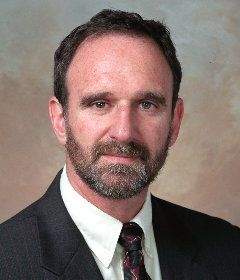
\includegraphics[width=\textwidth]{Martin-Hellman.jpg}
    \caption{Martin Hellman}
  \end{minipage}
  \hfill
  \begin{minipage}[hb]{0.3\textwidth}
    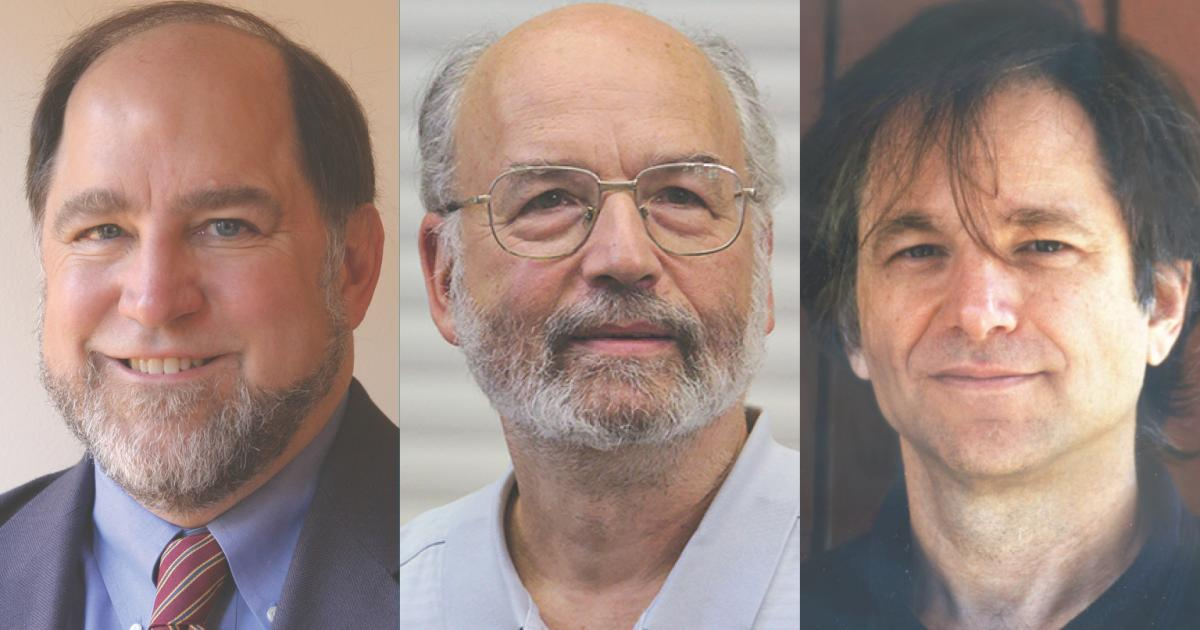
\includegraphics[width=\textwidth]{RSA.jpg}
    \caption{Rivet-Shamir-Adleman}
  \end{minipage}
  \hfill
  \begin{minipage}[hb]{0.3\textwidth}
    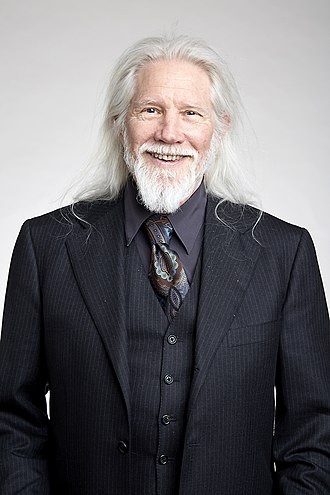
\includegraphics[width=\textwidth]{Diffle.jpg}
    \caption{Whitefield Diffle}
  \end{minipage}
\end{figure}

\section{RSA algorithm}
RSA(Rivet-Shamir-Adleman) is a public-key cryptosystem that is widley used for secure data transmission.The acronym "RSA" comes from the surname of Ron Rivest,Adi Shamir and Leonard Adleman, who publicly described the algorithm in 1977.In a public-key cryptosystem, the encryption key is public and distinct from the decryption key, which is kept secret(Private).An RSA user creates and publishes a public key based on two large prime number,along with an auxiliary value.The prime numbers are kept secret.Messages can be encrypted by anyone, via the public key,but can only be decoded by someone who knows the prime numbers.
The security of RSA relies on the practical difficulty of factoring the product of two large prime numbers, the "factoring problem".Breaking RSA encryption is know as the RSA problem.Whether it is as difficult as the factoring problem is an open question.There are no published methods to defeat the system if a large enough key is shared.RSA is a relatively slow algorithm.

Let's make this more concrete with an example. Take the prime numbers 13 and 7,their product gives us our maximum value of 91.Let's take our public encryption key to be the number 5. Then using the fact that we know 7 and 13 are the factors of 91 and applying an algorithm called the Extended Euclidean Algorithm, we get that the private key is the number 29 


\hspace{1cm}
\begin{centre}
\boxed{public \:key\:(e)\,:5\quad private\:key\;(d)\,:29\quad maximum\:key\:(n)\,:91}
\end{centre}

Let's use these values to encrypt the values to encrypt the message "CLOUD".
In order to represent a message mathematically we have to turn the letters into numbers.A common representation of the Latin alphabet is UTF-8.Each character corresponds to a  number.
\begin{figure}[h]
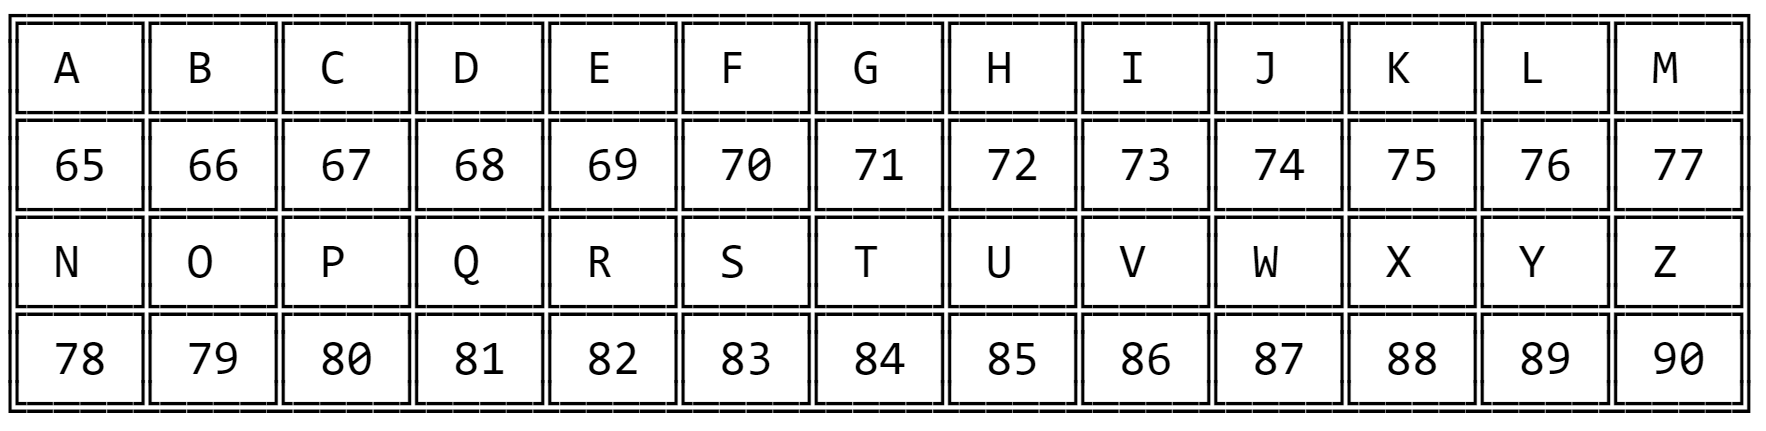
\includegraphics[width=10cm, height=2.5cm]{ASCII.png}
\centering
\end{figure}

Under this encoding,CLOUD is 67,76,79,85,68.Each of these digits are smaller than our maximum of 91,so we can encrypt them individually.Let's start with the first letter.
For C=67 we have to multiply it by itself 5(public key) times to get the encrypted value.

\begin{centre}
\boxed{\(Encrypted\:Data\:E\, = A^e*(mod n)\)}
\hspace{0.8cm}
\boxed{\(Decrypted\:Data\:D\,= L^d*(mod n)\)}
\end{centre}


\(Encrypted\:Data\:C\,=67^5mod91=58\) \hspace{0.6cm} \(Decrypted\:Data \:C\,=58^{29}mod91=67\)\\
\(Encrypted\: Data\: L\,=76^5mod91=20\) \hspace{0.6cm} \(Decrypted\:Data \:L\,=20^{29}mod91=76\)\\
\(Encrypted\: Data \:O\,=79^5mod91=53\) \hspace{0.6cm} \(Decrypted\:Data \:O\,=53^{29}mod91=79\)\\
\(Encrypted\: Data\: U\,=85^5mod91=50\) \hspace{0.6cm}\(Decrypted\:Data \:U\,=50^{29}mod91=85\)\\
\(Encrypted \:Data\: D\,=68^5mod91=87\) \hspace{0.6cm} \(Decrypted\:Data \:D\,=87^{29}mod91=68\)\\

So we can see that there no symmetric relation in keys so it will be harder to decrypt.

The Takeaway is that you can take a number,multiply it by itself a number of times to get a random-looking number,then multiply that number by itself a secret number of times to get back to the original number.
These factoring algorithms get more efficient as the size of the numbers being factored get larger.The gap between the difficulty of factoring large numbers and multiplying large numbers is shrinking as the number(The key's bit length) gets larger.As the resources available to decrypt numbers increase,the size of the keys need to grow even faster.This is not a sustainable situation for mobile and low-powered devices that have limited computational power.The gap between factoring and multiplying is not sustainable in the long term.

All this means is that RSA is not the ideal system for the system for the future of cryptography.In an ideal Trapdoor  Function,the easy way and the hard way get harder at the same rate with respect to the numbers in question

After the introduction of RSA and Diffie-Hellman, researchers explored other mathematics-based cryptographic solutions looking for other algorithms beyond factoring that would serve as good Trapdoor Functions. In 1985, cryptographic algorithms were proposed based on an esoteric branch of mathematics called elliptic curves.
\section{Elliptic curve Cryptography}
elliptic-curve cryptography is a approach to public key cryptography based on the algebraic stricture of elliptic curves over finite fields.ECC allows smaller keys compared to non-EC cryptography(based on plain Galois Fields) to provide equivalent security.The use of elliptic curve in cryptography was suggested by independently by Neal Koblitz and Victor S.Miller in 1985. Elliptic curve cryptography algorithms entered wide use in 2004 to 2005.

\begin{figure}[h]
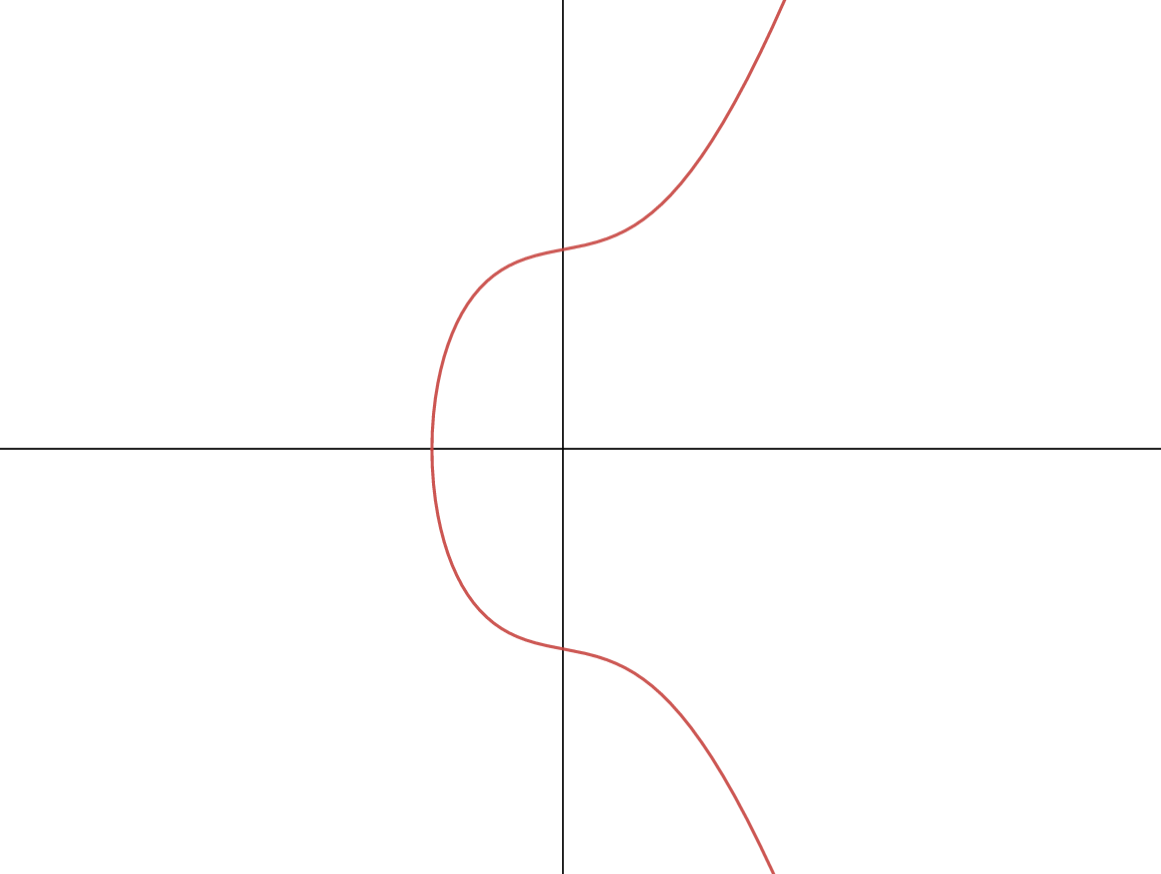
\includegraphics[width=10cm, height=3.3cm]{ECC.png}
 \caption{Elliptic Curve\:\(y^2=x^3+ax+b\)}
\centering
\end{figure}

Elliptic curves cryptography uses elliptic curves over the fintie field \(Z_{p}\)(where \(p\) is prime and \(p>3\)) or \(Z_{2m}\) (where the fields size p=2m).This means that the field is a square matrix of size \(p*p\) and the point on the curve is limited to integer coordinates within the field only.All algebric operation within the field (like point multiplication and addition) result in another point within the field.

\textbf{The Elliptic curve equation over the finite field \(Zp\)}

\hspace{4.5cm}
\begin{centre}
\boxed{\(y^2=x^3+ax+b(mod p)\)}
\end{centre}

\textbf{The Bitcoin curve(secp256k1) equation over the finite field \(Zp\)}

\hspace{4.5cm}
\begin{centre}
\boxed{\(y^2=x^3+7(mod p)\)}
\end{centre}

Unlike RSA,which uses for its key space the integers in the range[0...p-1](the field Zp),the ECC uses the points\{x,y\} within the Galois field Zp(where x and y are integers in the range[0...p-1]

\subsection{Mathematics}
Given a curve,E,defined along some equation in a finite field(such as E:\(y^2=x^3+ax+b\),point multiplicatioj is defined as the repeated addition of a point along that curve.denote as \(nP=P+P+P...+P\) for some scalar n and a point \(P=(x,y)\) that lies on  the curve,E.
\subsubsection{Point Operations}


\begin{figure}[hb]
  \centering
  \begin{minipage}[hb]{0.31\textwidth}
    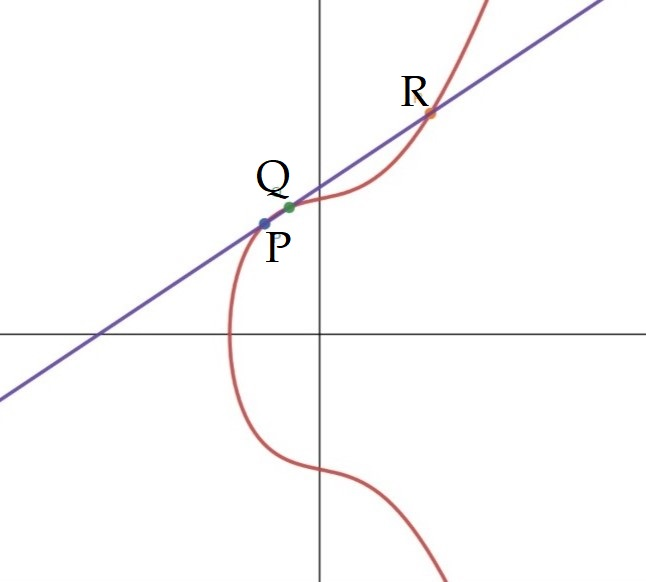
\includegraphics[width=\textwidth]{PQR1.jpeg}
    \caption{       \(P+Q+R=0\)}
  \end{minipage}
  \hfill
  \begin{minipage}[hb]{0.31\textwidth}
    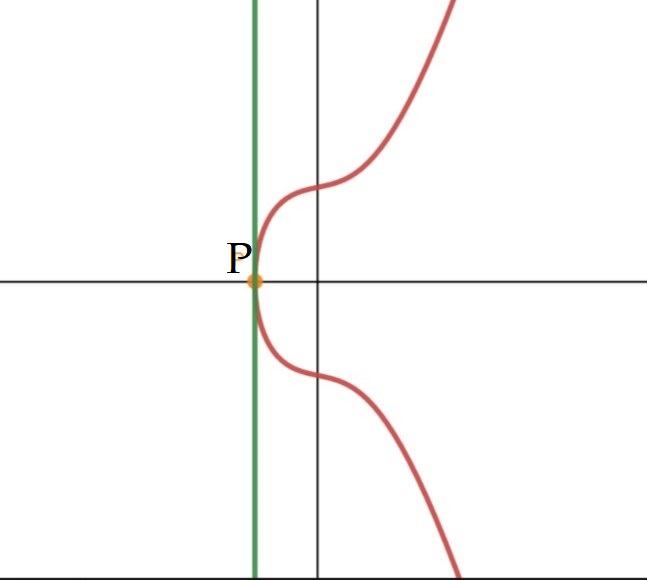
\includegraphics[width=\textwidth]{P.jpeg}
    \caption{  \(P+P+0=0\)}
  \end{minipage}
  
  \begin{minipage}[hb]{0.31\textwidth}
    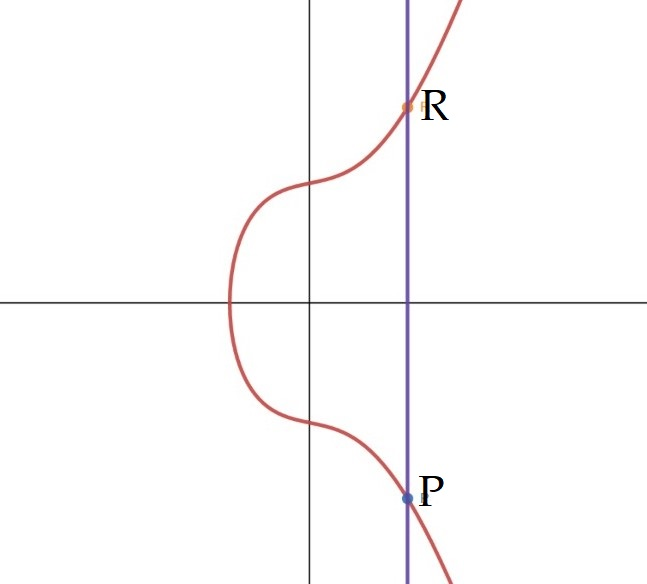
\includegraphics[width=\textwidth]{PR.jpeg}
    \caption{  \(P+R+0=0\)}
  \end{minipage}
  \hfill
  \begin{minipage}[hb]{0.31\textwidth}
    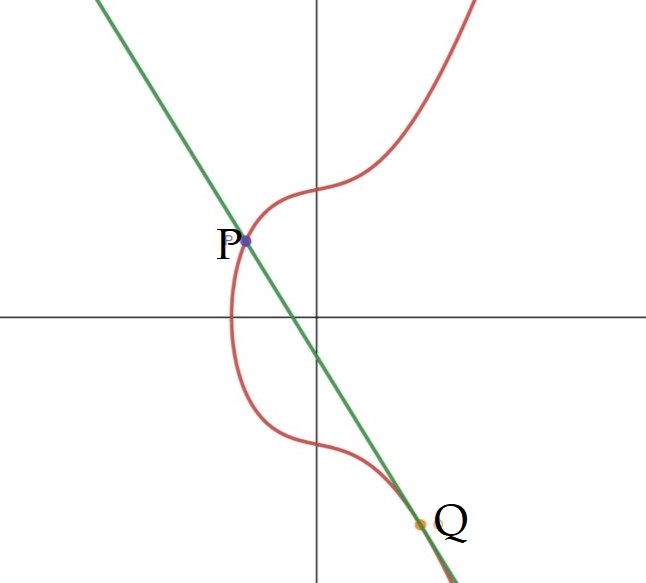
\includegraphics[width=\textwidth]{PQ.jpeg}
    \caption{  \(P+Q+Q=0\)}
  \end{minipage}
  \hfill
  
\end{figure}
\textbf{Point at Infinity}
\newline
Point at infinity \({\mathcal{O}}\) is the identity element of elliptic curve arithmetic.Adding it to ant point result in that other point,including adding point at infinity to itself.That is

\hspace{4cm}
\begin{centre}
\boxed{\({\mathcal{O}}+{\mathcal{O}}={\mathcal{O}}\)}
\newline
\end{centre}

\hspace{4cm}
\begin{centre}
\boxed{\({\mathcal{O}}+{\mathcal{P}}={\mathcal{P}}\)}
\end{centre}

\textbf{Point negation}
\newline
Point negation is finding such a point,that adding it to itself will result in point at infinity(\({\mathcal{O}}\)).

\hspace{3.9cm}
\begin{centre}
\boxed{\({\mathcal{P}}+({\mathcal{-P}})={\mathcal{O}}\)}
\end{centre}

For elliptic curves that is a point with same x coordinate but negated y coordinate:

\begin{centre}
\boxed{\((x,y)+(-(x,y))={\mathcal{O}}\)}
\end{centre}
\begin{centre}
\boxed{\((x,y)+(x,-y))={\mathcal{O}}\)}
\end{centre}
\begin{centre}
\boxed{\((x,-y)=-(x,y)\)}
\end{centre}

\textbf{Point addition}
\newline
With 2 distinct points,$P$ and $Q$,addition is defined as the negation of the point resulting from the intersectio of the curve,$E$,and the straight line defined by the points $P$ and $Q$ giving the point,$R$

\hspace{4.3cm}
\begin{centre}
\boxed{$P$\:+ \:$Q$ \:= \:$R$}
\end{centre}

Assuming the elliptic curve,$E$, is given by \(y^2=x^3+ax+b\), this can be calculated as:
\hspace{3cm}
\begin{center}
    \boxed{\lambda=\frac{y_{q}-y_{p}}{x_q-x_p}}
\end{center}
\hspace{2.5cm}
\begin{centre}
\boxed{x_{r}=\lambda^2-x_{p}-x_{q}}
\end{centre}
\begin{centre}
\boxed{y_{r}=\lambda((x_{p}-x_{r})-y_{p}}
\end{centre}

These equations are correct when neither point is the point at infinity,{\mathcal{O}},and if the points have diffrent x coordinates(they're not mutual inverses).This is important for the Elliptic curve digital singature algorithm(ESDSA) where the hash value could be zero.

\textbf{Point doubling}
\newline
Where the point $P$ and $Q$ are coincident(at same coordinate),addition is similar,except that there is no well-defined straight line through $P$,so the operation is closed using limiting case,the tangent to the curve,$E$,at $P$.
This is calculated as above,taking derivatives
\begin{center}
    \boxed{{\frac{\partial E}{\partial x}}/{\frac{\partial E}{\partial y}}}
\end{center}
\begin{center}
    \boxed{\lambda=\frac{3x_{p}^2+a}{2y_{p}}}
\end{center}
where a is from the defining equation of the curve,$E$,above.

\end{document}
